\documentclass{article}
\usepackage{v-equation}
\vgeometry[8][4.5][0]
\begin{document}

\vspace*{\fill}
\begin{center}
\Huge{\textbf{IIT-JEE}}\\
\texttt{\textbf{[2022]}}
\end{center}
\vspace*{\fill}

\begin{center}
\begin{tikzpicture}
[scale=1.0, line width=1.0 mm, cap=round, black]
	\tzline(-7, 0)(7, 0)
	\tzellipse(0, 0)(0.4cm and 3cm)
	\tzline+[ultra thick] (-5, 0)(120:1)
	\tzanglemark(0, 0)(-5, 0)($(-5, 0)+(120:1)$){$\dfrac{2\pi}{3}$}[r]
	\tzline+[ultra thick] (6, 0)(-120:2)
	\tzanglemark(0, 0)(6, 0)($(6, 0)+(-120:2)$){$\alpha$}
	\tzline[|<->|]<0, -0.5>(-5, 0)(0, 0){$\dfrac{40}{3}$}[mb]
	\tzline+[|<->|]<-0.5, 0>($(6, 0)+(-120:2)$)(0, 2*sin{60}){$\dfrac{30\sqrt{3}}{13}$}[ml]
\end{tikzpicture}
\end{center}
\vspace*{\fill}

\end{document}